\documentclass{article}
\usepackage[utf8]{inputenc}
\usepackage[russian]{babel}
\usepackage{graphicx}
\usepackage{titlesec}
\usepackage{indentfirst}
\setlength{\parskip}{1ex plus 0.5ex minus 0.2ex}
\usepackage{geometry}
\geometry{verbose,a4paper,tmargin=2cm,bmargin=2cm,lmargin=2.5cm,rmargin=1.5cm}

\titleformat{\section}
{\normalfont\Large\bfseries}{\S\thesection}{1em}{}

\title{Лекции Информационная безопасность}
\author{ Колесов В.А. }
\date{Ноябрь 2018}


\begin{document}

\maketitle

\newpage

\section{ Основные понятия и определения}
\subsection{ Информационная безопасность и защита информации }
\textit{Информационная безопасность} - это состояние защищённости информации, обеспечивающее
сохранность информации от случайных или преднамеренных действий искусственного или
естественного характера, а также обеспечение сохранности поддерживающей инфраструктуры. Под поддерживающей инфраструктурой понимаются: носители информации(бумажные или электронные), информационные системы(базы данных), серверы, линии связи, энергоснабжение, обслуживающий персонал и.т.д.


\textbf{Определение 1}
\textit{Защита информации} - это процесс направленный на обеспечение информационной безопасности.


\textbf{Определение 2}
\textit{Защита информации} - комплекс мероприятий направленных на обеспечение сохранности информации и поддерживающей инфраструктуры.

\subsection{Составляющие информационной безопасности:}
К составляющим информационной безопасности относится:
\begin{itemize}
\item конфиденциальность;
\item доступность;
\item целостность;
\item аппелируемость.
\end{itemize}

\textit{Конфиденциальность} - это свойство информации при котором она защищена от несанкционированного доступа.

\textit{Несанкционированный доступ} - это получение или раскрытие информации без необходимых на то полномочий.

\textit{Конфиденциальность} является наиболее проработанной составляющей информационной безопасности, определяется моделями доступа к данным и законодательными актами, классифицирующими уровни конфиденциальности. Основное средство защиты конфиденциальности - система шифрования. Свойство конфиденциальности является приоритетным в случаях когда речь идёт о защите: государственной тайны, персональных данных,  интернет-трафика, коммерческой или служебной тайны.

\textit{Доступность} - свойство информации, гарантирующее получение запрашиваемой легальным путём информации в установленные временные рамки. Свойство доступности является приоритетным для получения общедоступной информации, предоставляемой интернет-сервисами, а также в системах управления принятием решений. Основные средства обеспечения доступности: наращивание вычислительных мощностей, увеличение полосы пропускного канала связи, создание резервных серверов, репликация баз данных, а также создание резервных источников питания.

\textit{Целостность} - это свойство информации, при котором гарантируется нахождение информации в согласованном состоянии.Транзакция переводит базу данных из одного согласованного состояния в другое. Транзакция является атомарной (выполняется полностью). Свойство целостности является приоритетным, когда проводится обработка информации с использованием баз данных.

\textit{Аппелируемость} - это фиксирование факта обработки и создания информации для обеспечения неразрывных связей между субъектом
действия(пользователь, учётная запись) и обрабатываемой информацией. Основное средство - цифровая подпись. Свойство целостности является приоритетным в случае установления авторами прав либо привлечения к ответственности за создание ложной информации.

\section{ Угрозы информационной безопасности}
\subsection{ Основные определения }
\textbf{Определение 1}
Под \textit{угрозой} понимается потенциально возможное событие, действие (воздействие), процесс или явление, которые могут привести к нанесению ущерба чьим-либо интересам.

\textbf{Определение 2}
\textit{Угроза} - вероятность того, что кто-либо может воспользоваться уязвимостью.
\subsection{Классификация угроз}
\begin{itemize}
\item По природе возникновения:
\begin{itemize}
\item естественные;
\item искусственные.
\end{itemize}
\item По степени преднамеренности:
\begin{itemize}
\item случайные(халатность, ошибка, природные явления);
\item преднамеренные.
\end{itemize}
\item По источнику угроз:
\begin{itemize}
\item природная среда(магнитные бури, бедствия и.т.п.);
\item человек(методы социального инжиниринга);
\item программно-аппаратное обеспечение(отказ в работе ПО или АО).
\end{itemize}
\item По положению источника угроз:
\begin{itemize}
\item вне контролируемой зоны(периметра безопасности);
\item внутри контролируемой зоны(периметра безопасности);
\item внутри информационной системы.
\end{itemize}
\item По степени зависимости от работы автоматизированной системы:
\begin{itemize}
\item независимо от активности системы(вскрытие информации);
\item в процессе обработки данных(заражение и распространение вируса).
\end{itemize}
\item По степени воздействия на систему:
\begin{itemize}
\item пассивные - не меняют структуру и содержание системы(копирование данных, прослушка);
\item активные - вносят изменение в структуру данных(троян).
\end{itemize}
\item По этапам доступа пользователей к информационным ресурсам:
\begin{itemize}
\item угрозы, на этапе доступа к ресурсам (несанкционированный доступ);
\item угрозы, после разрешения доступа к ресурсам(несанкционированное или некорректное использование ресурсов).
\end{itemize}
\item По способу доступа к ресурсам системы:
\begin{itemize}
\item угрозы, использующие стандартные пути для доступа к ресурсам;
\item угрозы, использующие скрытые, нестандартные пути(недокументированные возможности).
\end{itemize}
\item По месту расположения информации, обрабатываемой в системе:
\begin{itemize}
\item угрозы доступа к информации на внешних носителях;
\item угрозы доступа к информации в оперативной памяти;
\item угрозы доступа к информации в каналах связи;
\item угрозы доступа к информации на терминале либо вспомогательном устройстве.
\end{itemize}
\item По составляющей информационной безопасности, на которую направлена угроза:
\begin{itemize}
\item на \textit{целостность} - угроза направлена на искажение информации, которая приведёт к нарушению работы системы или к изменению (уничтожению) данных;
\item на \textit{конфиденциальность} - целенаправленное действие нарушителя(служащий, посетитель, конкурент), мотивированного недовольством карьерным положением, материальным интересом, конкурентной борьбой, повышением самооценки;
\item на \textit{доступность} - угроза направлена на создание ситуаций, при которых постоянно или временно снижается работоспособность системы, либо блокируется доступ к ресурсам(DOS).
\end{itemize}
\end{itemize}
\section{ Средства защиты информации}
\subsection{ Классификация }
\begin{center}
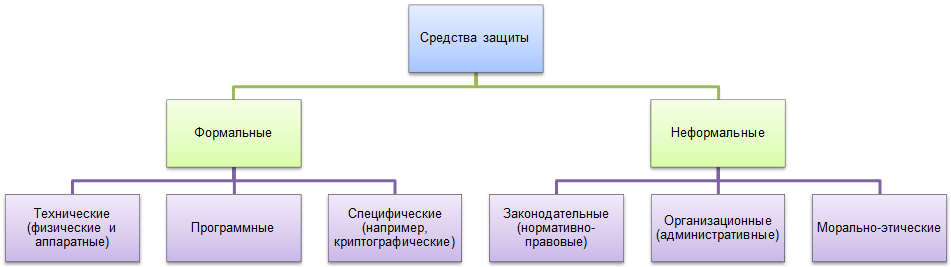
\includegraphics[width=16cm,height=4cm]{sredstvaZI.png}
\end{center}
\begin{itemize}
\item \textbf{Формальные средства защиты} (выполняют защитные функции строго по заранее предусмотренной процедуре без участия человека)
\begin{itemize}
\item \textit{Физические} - механические, электрические, электромеханические, электронные, электронно-механические и тому подобные устройства и системы, которые функционируют автономно от информационных систем, создавая различного рода препятствия на пути дестабилизирующих факторов (замок на двери, жалюзи, забор, экраны);
\item \textit{технические(аппаратные)} - механические, электрические, электромеханические, электронные, электронно-механические, оптические, лазерные, радиолокационные и тому подобные устройства, встраиваемые в информационных системах или сопрягаемые с ней специально для решения задач защиты информации;
\item \textit{программные} - пакеты программ, отдельные программы или их части, используемые для решения задач защиты информации. Программные средства не требуют специальной аппаратуры, однако они ведут к снижению производительности информационных систем, требуют выделения под их нужды определенного объема ресурсов и т.п;
\item  \textit{специфические} - криптографические методы. В информационных системах криптографические средства защиты информации могут использоваться как для защиты обрабатываемой информации в компонентах системы, так и для защиты информации, передаваемой по каналам связи. Само преобразование информации может осуществляться аппаратными или программными средствами, с помощью механических устройств, вручную и т.д.
\end{itemize}
\item \textbf{Неформальные средства защиты}(регламентируют деятельность человека)
\begin{itemize}
\item \textit{законодательные} – законы и другие нормативно-правовые акты, с помощью которых регламентируются правила использования, обработки и передачи информации ограниченного доступа и устанавливаются меры ответственности за нарушение этих правил. Распространяются на всех субъектов информационных отношений. В настоящее время отношения в сфере информационной безопасности регулируются более чем 80 законами и нормативными документами, иногда достаточно противоречивыми.
\item \textit{организационные} - организационно-технические и организационно-правовые мероприятия, осуществляемые в течение всего жизненного цикла защищаемой информационной системы (строительство помещений, проектирование информационных систем, монтаж и наладка оборудования, испытания и эксплуатация информационных систем). Другими словами – это средства уровня организации, регламентирующие перечень лиц, оборудования, материалов и т.д., имеющих отношение к информационным системам, а также режимов их работы и использования. К организационным мерам также относят сертификацию информационных систем или их элементов, аттестацию объектов и субъектов на выполнение требований обеспечения безопасности и т.д.
\item \textit{морально-этические} - сложившиеся в обществе или в данном коллективе моральные нормы или этические правила, соблюдение которых способствует защите информации, а нарушение приравнивается к несоблюдению правил поведения в обществе или коллективе, ведет к потере престижа и авторитета. Наиболее показательный пример – кодекс профессионального поведения членов Ассоциации пользователей ЭВМ США.
\end{itemize}
\end{itemize}
\section{ Правовые основы информационной безопасности в Российской Федерации }
\subsection { Законодательная база }
Законодательная база включает в себя пакет федеральных законов, указов президента, постановлений правительства, межведомственных руководящих документов и стандартов. Основополагающими является конституция и концепция национальной безопасности. В конституции гарантируется права гражданина, например:
\begin{itemize}
\item статья 23 - тайна переписки, телефонных разговоров, почтовых и телеграфных сообщений;
\item статья 29 - право свободно искать, получать, передавать и распространять информацию законным способом.
\end{itemize}

Концепция национальной безопасности принята в январе 2000 года и определяет:
\begin{itemize}
\item реализацию конституционных прав граждан в сфере информационной деятельности;
\item совершенствование национальной инфраструктуры для защиты информации;
\item противодействие угрозе конфликтов в информационной сфере.
\end{itemize}

\textit{Государственная тайна} - это защищаемые государством сведения в области военной, внешнеполитической, экономической, разведывательной, контрразведывательной, оперативно-розыскной деятельности, распространение которых может нанести ущерб безопасности Российской Федерации.

\textit{Гриф секретности} - реквизиты, свидетельствующие о степени секретности сведений, содержащихся на носителе, предоставляемые либо на самом носителе, либо на сопроводительной документации. Например, гриф ДСП - для служебного пользования.

\subsection{ Закон 149 }
Закон 149 - об информации, информационных технологиях, информационной безопасности является одним из основных базовых законов в области защиты информации, регламентирует отношения возникающие при формировании и использовании информационных ресурсов в Российской Федерации, защищает информацию и права субъектов. Участвующих в информационных отношениях.

Основные задачи закона 149:
\begin{itemize}
\item предотвращение утечки, хищения, утраты, несанкционированных действий с информацией;
\item сохранение полноты, достоверности, целостности информации;
\item сохранение возможности управления процессом обработки;
\item обеспечение конституционных прав граждан на сохранение личной тайны и конфиденциальности персональной информации;
\item сохранение секретности информации в соответствии с законодательством;
\item соблюдение авторских прав на программно-информационную продукцию.
\end{itemize}
\section { Криптография }
\subsection{ Основные определения }
\textit{Криптография} - наука, которая исследует математические особенности шифрования и разрабатывает алгоритмы для сокрытия информации от несанкционированного доступа.

\textit{Криптоанализ} - наука, изучающая стойкость шифра к различным способам вскрытия, не зная ключа.

\textit{Криптология} - это совокупность криптографии и криптоанализа.

\textit{Стеганография} - наука, которая изучает возможности сокрытия полезной информации в большом объёме обычной информации. Особенностью является то, что скрывается не только сообщение, но и сам факт наличия сообщения.

\subsection{ Классификация шифров }
\begin{itemize}
\item по области применения:
\begin{itemize}
\item шифры ограниченного исполнения(позируются на правиле, что знание алгоритма шифрования позволяют ускорить процесс вскрытия шифра;
\item шифры общего пользования(стойкость основана на секретности ключа и сложности подбора для криптоанализа).
\end{itemize}
\item по особенностям алгоритма шифрования:
\begin{itemize}
\item симметричное - одноключевое. Шифры замены, шифры перестановки, аддитивные шифры, квантовые шифры;
\item ассиметричное - детерминированные, вероятностные. В детерминированных шифрах при шифровании одного и того же сообщения одним и тем же ключом всегда будет получаться один и тот же шифротекст. В вероятностных шифрах в процедуре шифрования используется дополнительная случайная величина (число) - в результате при шифровании одного и того же исходного сообщения одним и тем же ключом могут получиться разные шифротексты, которые при расшифровке дадут один и тот же результат (исходное сообщение).
\end{itemize}
\item по количеству бит в однотипной процедуре шифрования:
\begin{itemize}
\item потоковые(процедура преобразования применяется к отдельному байту сообщения);
\item блочные(процедура преобразования применяется к блоку байт сообщения).
\end{itemize}
\end{itemize}
\end{document}
